\documentclass{article}
\usepackage[utf8]{inputenc}
\usepackage[russian]{babel}
\usepackage[left=2cm,right=2cm,
top=2cm,bottom=2cm,bindingoffset=0cm]{geometry}
\usepackage{graphicx}
\usepackage{amsmath}
\usepackage{float}
\usepackage{listings}
\usepackage{url,textcomp}
\date{2019 г.}
\author{Кондратенко Федор, гр 13632/1}
\setlength{\parindent}{0pt}
\setlength{\parskip}{5pt plus 2pt minus 1pt}
\frenchspacing
\title{Отчет по изготовлению сложной детали в Simulink}
\begin{document}
	\maketitle
	Требовалось создать блок-схему,моделирующую вращающуюся деталь на стержне:
	\begin{figure}[H]
		\centering
		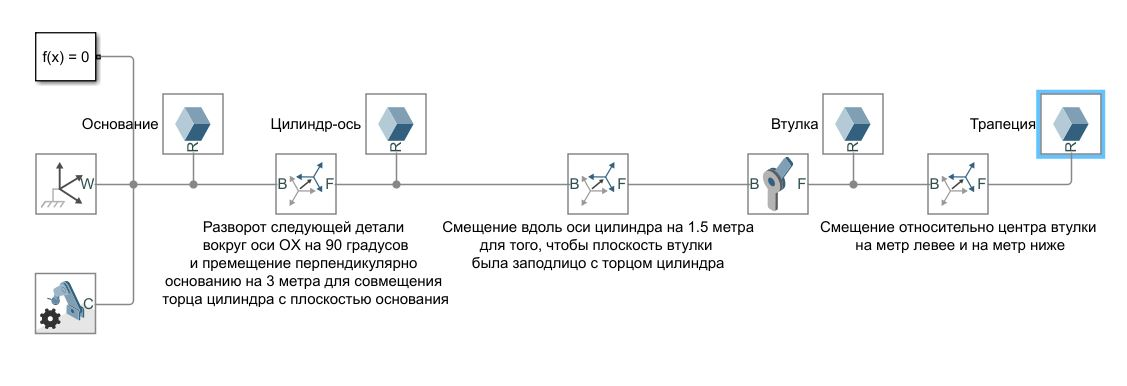
\includegraphics[width=1\linewidth]{model}
		\caption{Блок-схема; под каждым поворотом сделано примечание}
		\label{fig:model}
	\end{figure}
	Результат моделирования:
	\begin{figure}[H]
		\centering
		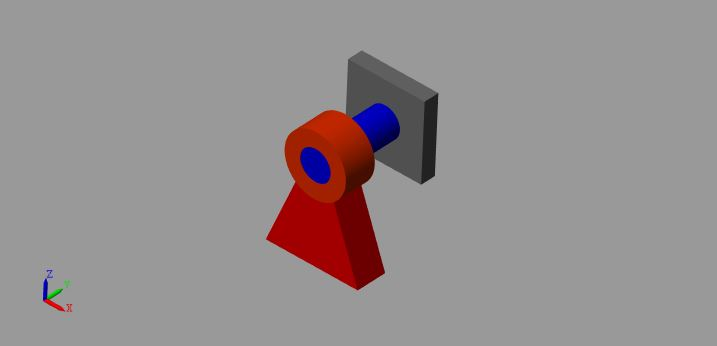
\includegraphics[width=1\linewidth]{3d}
		\caption{Результат моделирования}
		\label{fig:3d}
	\end{figure}
	Данная модель создана из четырех деталей:
	\begin{figure}[H]
		\centering
		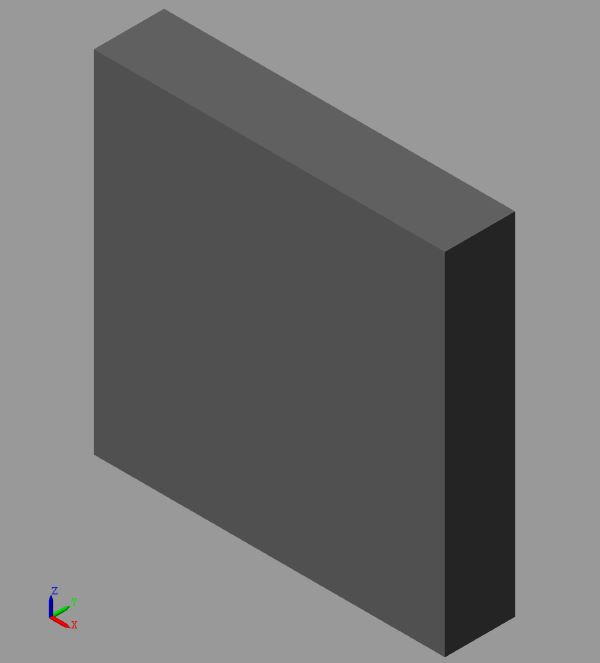
\includegraphics[width=0.7\linewidth]{base}
		\caption{Основание -- параллелепипед с параметрами 5x5x1}
		\label{fig:base}
	\end{figure}
	\begin{figure}[H]
		\centering
		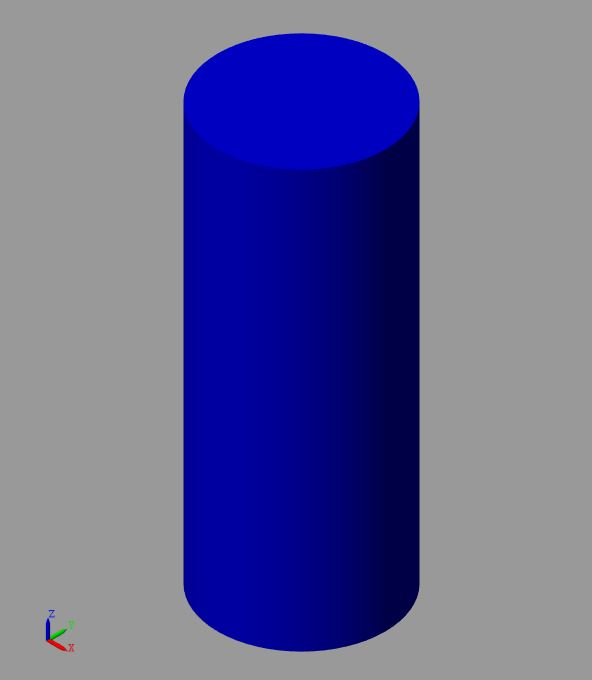
\includegraphics[width=0.7\linewidth]{cylinder}
		\caption{Ось, которая крепится к основанию, представляет собой цилиндр радиусом 1 метр и длиной 5 метров}
		\label{fig:cylinder}
	\end{figure}
	\begin{figure}[H]
		\centering
		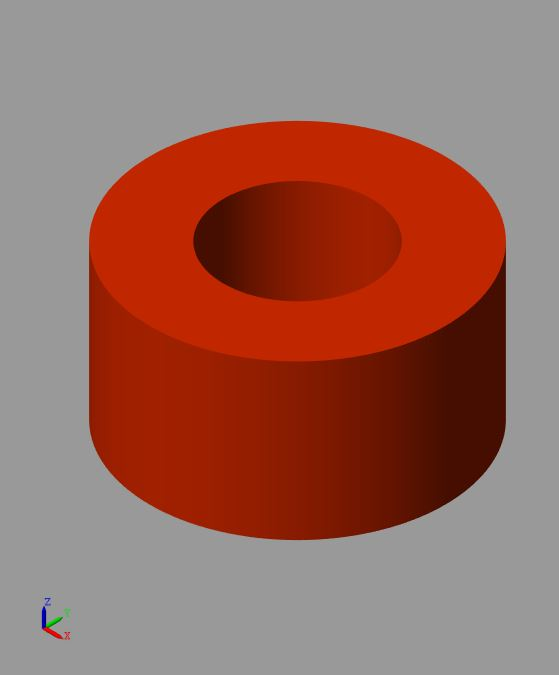
\includegraphics[width=0.7\linewidth]{vtulka}
		\caption{Втулка, которая свободно вращается на оси, является телом вращения, радиус внутренней полости -- 1 метр, внешний радиус -- 2 метра}
		\label{fig:vtulka}
	\end{figure}
	\begin{figure}[H]
		\centering
		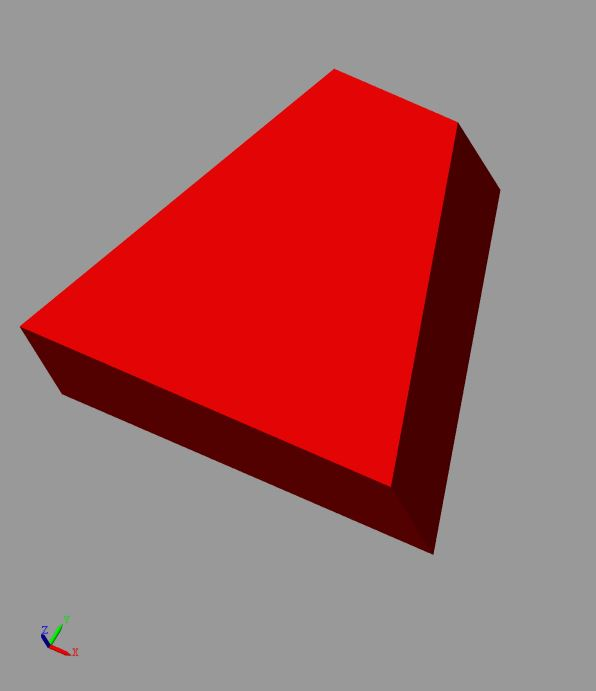
\includegraphics[width=0.7\linewidth]{trap3d}
		\caption{Маятник, который жестко соединен с втулкой. Имеет форму трапеции}
		\label{fig:trap3d}
	\end{figure}
	\begin{figure}[H]
		\centering
		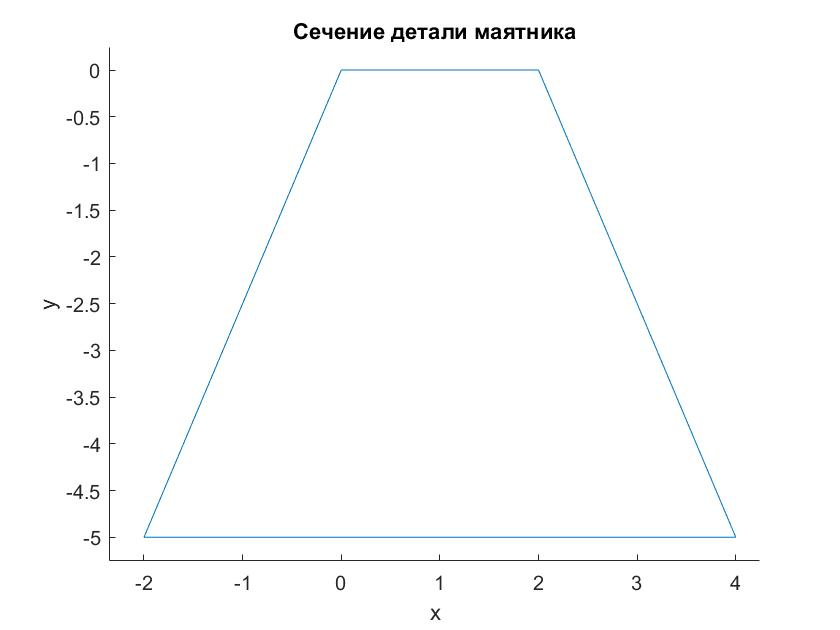
\includegraphics[width=0.7\linewidth]{trap}
		\caption{Сечение маятника}
		\label{fig:trap}
	\end{figure}
	
\end{document}